%===================================== CHAP 2 =================================

\chapter{Theory}

The primary purpose of the circulatory system is to deliver oxygenated blood to tissue, where the supply of oxygen is the product of flow and oxygen content\cite{RN11}. The body has developed innate self-regulatory systems to maintain appropriate blood flow and tissue perfusion. In a healthy individual, hemodynamic parameters fluctuate as autoregulatory mechanisms keep the cardiovascular system within a stable region.

The hemodynamic parameters, such as the \textit{systemic vascular resistance} (SVR) and \textit{compliance}, can be used to create a simple but robust model of the arterial system. Analogous to a parallel RC circuit, the diameter of the veins decides the systemic resistance that must be overcome for blood to pass through the arterial system, while compliance represents the ability of the arterial system to distend as a function of the slow changes in pressure. This kind of lumped model used for representing the arterial system is known as a Windkessel (WK) model.

In a septic patient, the autoregulatory mechanisms, as well as other efforts to maintain homeostasis, are impaired. The distinguishable slow autoregulatory changes in the arterial parameters will then be less stable, causing noticeable differences in the impedance of the arterial system.


\section{Sepsis}

Sepsis is a serious and crippling clinical condition that significantly changes the lives of those affected. The word septic originates from the old Latin term meaning rotten, in the same way, sepsis is derived from the Greek word for "decomposition" or "decay" \cite{RN3}. Something being in a state of \textit{shock} means decreased tissue oxygenation (reduced oxygen delivered to cells as a result of problems with the circulatory system) and low blood pressure. Combining the terms one gets something rotten, or infected material, causing a decreased oxygenation of organ tissue. 

\subsection{Epidemiology}

\begin{table}[t!]
  \begin{center}
    \caption{Criteria for the systemic inflammatory response syndrome (SIRS), defined as fulfilling two or more of the listed criteria. \cite{RN4}}
    \label{tab:SIRS}
    \begin{tabular}{l|c} % <-- Alignments: 1st column left, 2nd middle and 3rd right, with vertical lines in between
      \textbf{Criterion} & \textbf{Value} \\
      \hline
      Temperature & $>38^\circ C$ or $<36^\circ C$\\
      Heart rate & $>90$ bpm \\ 
      Respitory rate & $>20$ or PaCO2$<32$ mmHg \\
      White bloodcell count & $>12,000/\mu L$ or $<4,000/\mu L$, or $<10\%$ band 
    \end{tabular}
  \end{center}
\end{table}

Sepsis is most commonly caused by a bacterial infection, but it may also be fungal, viral, or protozoan \cite{RN2}. In 1991 a universal and easy-to-apply set of clinical parameters were invented during a consensus conference working toward identification and treatment of the disease. This set of parameters is known by the term “systemic inflammatory response syndrome” (SIRS) \cite{RN6}. SIRS affects the whole body and is defined by the presence of two or more of the criteria listed in table \ref{tab:SIRS}. The diagnosis of sepsis requires both evidence of an infection along with the patient being in a SIRS disease state. Sepsis can be divided into three stages: sepsis, severe sepsis, and septic shock. The SIRS criteria need to be present before the doctor can diagnose sepsis. Severe sepsis is a more severe stage of sepsis, associated with hypotension, hyperfusion, or organ dysfunction.\cite{RN8} Septic shock is the final and most severe stage of sepsis and is associated with the same cardiovascular and organ deviance as for severe sepsis, but at critical levels, which can cause acute failure of multiple organs. Septic shock is defined as sepsis associated with hypotension and perfusion abnormalities despite the provision of adequate fluid (volume) resuscitation \cite{RN8}. 


\subsection{Pathophysiology}\label{sect:pathophysiology}

Sepsis starts out as a typical inflammatory response to an infection. The body's immune system reacts to invading pathogens in several ways. The initial response happens when white blood cells, also called leukocytes, encounter any invading antigen and immediately activates. When white blood cells activate, they recruit more white blood cells to eradicate the harmful organism. Since the infected material is usually located in the interstitial tissue, and not in the bloodstream, the white blood cells release molecules like Nitrous Oxide (NO) \cite{RN9}. The nitrous oxide signals the surrounding smooth muscle to relax, resulting in vasodilation. This increase in vessel diameter causes a decrease in systemic vascular resistance, which means an increase in blood flow to the area in combination with increased permeability, or leakiness, of the vessel walls \cite{RN10}. Both of these factors help the immune cells to reach the affected area. With the increased leakiness, fluid will build up in the tissue, making it difficult for red blood cells to oxygenate the surrounding tissue. This starvation of oxygen is essentially what causes a septic shock. 

The goal of the white blood cells is to get rid of the infected material by releasing lytic enzymes and reactive oxygen species whose job it is to damage the pathogen \cite{RN13}. These enzymes end up damaging the blood vessels as well as the pathogen. Whenever a blood vessel is damaged, a physiological process called hemostasis changes the blood from a fluid liquid to a more gelatinous state. Hemostasis slows down the blood flow and forms blood clots to prevent blood from spilling into extravascular space \cite{RN12}. The coagulation factors cannot keep up with the ruptures, and blood clots will start blocking blood flow to any parts of the body, including limbs and organs. This vicious cycle caused by the body's inability to restore homeostatic conditions, contributing to multiple organ dysfunctions is called Disseminated Intravascular Coagulation (DIC) \cite{RN14}. 

To sum up the two main cardiovascular occurrences, from initial inflammatory response to septic shock: 
 \begin{enumerate}
    \item White blood cells release enzymes and reactive oxygen species to fight the infection.
    \item Increased relase of NO causes an increase in vasodilation to reach pathogens in the interstitual tissue $\longrightarrow$ increased permeability and leakiness.
   \item The reactive oxygen species will cause the vessels to rupture, further increasing the leakiness.
   \item By now, fluids have built up in the tissue, making it difficult to oxygenate tissue.
   \item Hemostasis initiated by the ruptures creates blood clots all over the vascular system, obstructing blood flow, making it even harder to oxygenate tissue and critical organs.
   \item The incapability to oxygenate will lead to varying degrees of organ failure and tissue death.
\end{enumerate}

The main takeaway is that there are hemodynamic changes in parameters such as pressure, blood flow, venous resistance and dilation, and other parameters as the sepsis develops. During these events, the body's ability to autoregulate and maintain homeostasis is severely deprecated.



\section{hemodynamics}\label{sect:hemodynamics}

Hemodynamics is the dynamics that govern blood flow. Like a control system controlling hydraulic circuits, e.g., pumps and pipes, the circulatory system is kept in stable condition by homeostatic control mechanisms. The heart is the pump of the circulatory system, pumping oxygen-rich blood to organs and tissue through contracting and relaxing. During the cardiac cycle, the period of contraction is called systole, and the period of relaxation is called diastole. The pulsating characteristics of the hemodynamics stem from this hydrostatic pressure gradient and the cardiovascular impedance. As blood is ejected into the aorta and to the rest of the arterial system, the elastic fibers of the arteries will help maintain the pressure and flow gradients as they dilate and resist any immediate changes. The content of this and the following section is mostly taken from "Snapshots of Hemodynamics: An Aid for Clinical Research and Graduate Education" \cite{RN11}.


\subsection{Blood pressure and velocity}

\begin{figure}[t!]
    \centering
    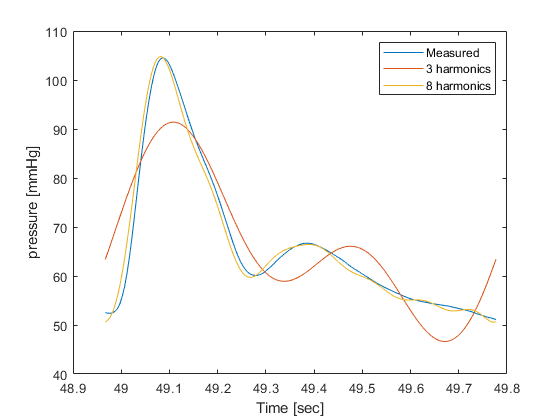
\includegraphics[width=0.6\textwidth]{fig/theory/reconstruct_pressure.png}
    \caption{Measured pulsatile pressure vs. reconstructed pressure using the harmonic frequencies}
    \label{fig:reconstruct_pressure}
\end{figure}{}

As the pulsatile flow and pressure are a result of a sudden change in pressure and the impedance of the arterial system, it is expected to have a periodic character, which is what we refer to as the cardiac cycle. Milnor WR. in the book "Hemodynamics" \cite{RN15} states that the flow and pressure profile is a complex waveform built up of various harmonics, given by a series of sine waves produced by the heart pumping blood through the different chambers of the heart. These waveforms can be represented as superpositions of several harmonics:
\begin{equation}
    p = \sum_{n=0}^{N-1}p_ne^{j\omega_nt} 
    \hspace{0.2cm}\textrm{and}\hspace{0.2cm}
    q = \sum_{n=0}^{N-1}q_ne^{j\omega_nt} 
    \label{eq:pressure&flow}
\end{equation}
where $q_n$ and $p_n$ are the complex Fourier components given by the angular frequencies $\omega_n$. The actual flow and pressure can then be extracted as the real part of the complex functions in equation \ref{eq:pressure&flow}. If one were able to obtain the frequency response of either pressure or flow, one would be able to reconstruct the signal without too much deviation by using its first few harmonics. Figure \ref{fig:reconstruct_pressure} demonstrates how much information that is held within the first harmonics of one blood pressure measurement. One could successfully reconstruct the whole signal by simply employing the first 8-10 harmonics.


\subsection{Impedance}\label{sect:impedance}

The impedance of a segment of the vascular system is the relation between the local difference in pressure and flow. It is a measure of the system's ability to resist an immediate motion of fluids when subjected to an increase in pressure. As explained in the previous section, both pressure and flow can be represented by a linear combination of their harmonics. The vascular impedance is defined as the ratio between the complex pressure ($P$) to complex flow ($V$) for the harmonic frequencies:
\begin{equation}
    Z(\omega) = \frac{P(\omega)}{V(\omega)} 
    \label{eq:impedance}
\end{equation}
 Figure \ref{fig:impedance} shows the magnitude of the impedance as a function of its harmonic frequencies from a cardiac cycle\footnote{If the original sequence is one cycle of a periodic function, the digital Fourier transform provides all the non-zero values of one DTFT cycle, and the frequency vector is spaced by multiples of the harmonic frequency ($\Delta f=\frac{f_s}{N_{fft}}$)}. In theory, the magnitude should approach a constant value, and the phase angle close to zero, which is the contribution of the characteristic impedance \cite{RN15}. Without reflections in the arterial system, the input impedance would equal characteristic aortic impedance, and the pressure and flow would have the same wave shape. For low frequencies, the reflections at the periphery, the 'diffuse reflections,' are large and cause the impedance to be high. At high frequencies, local 'distinct reflections' play a role, and they determine the oscillations in the impedance about the characteristic impedance. At zero frequency is the SVR, while the first harmonic provides a measure of the arterial compliance.

\begin{figure}[t!]
    \centering
    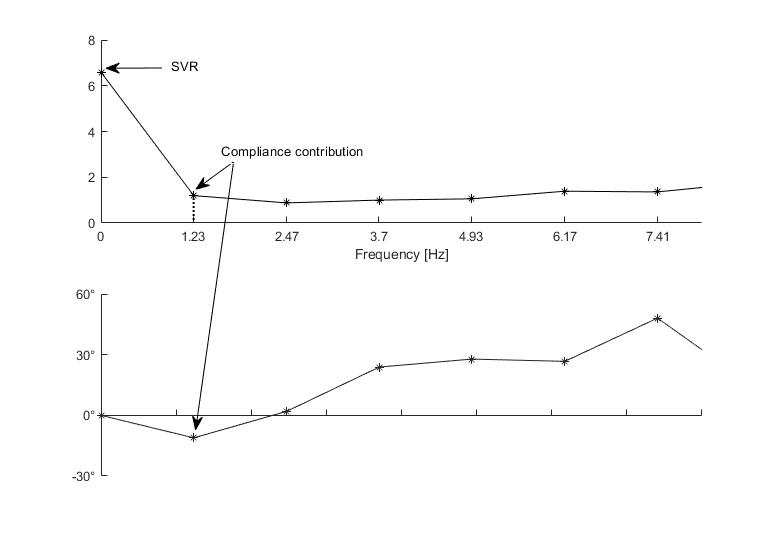
\includegraphics[width=0.8\textwidth]{fig/theory/impedance.png}
    \caption{Impedance magnitude and phase of the pressure plot shown in figure \ref{fig:reconstruct_pressure} as a function of the harmonic frequencies. The magnitude at zero frequency is the SVR, and the steady decrease in magnitude is contributed by the arterial compliance.}
    \label{fig:impedance}
\end{figure}{}

The compliance of the cardiovascular system is due to the elastic properties of the cardiovascular system. The vascular tissue is mainly composed of elastin, smooth muscle and collagen \cite{RN11}\cite{RN17}. Elastin fibers are highly extensible and demonstrate viscoelastic properties, i.e. a rapidly applied force to the material will require more force to achieve the same widening as a purely elastic material. The vessel wall's ability to expand and contract as pressure increase or decrease is known as compliance ($C$), and is quantified as a change in volume ($\Delta V$) divided by a change in pressure ($\Delta P$) \cite{RN15}. 

\begin{figure}[h!]
    \centering
    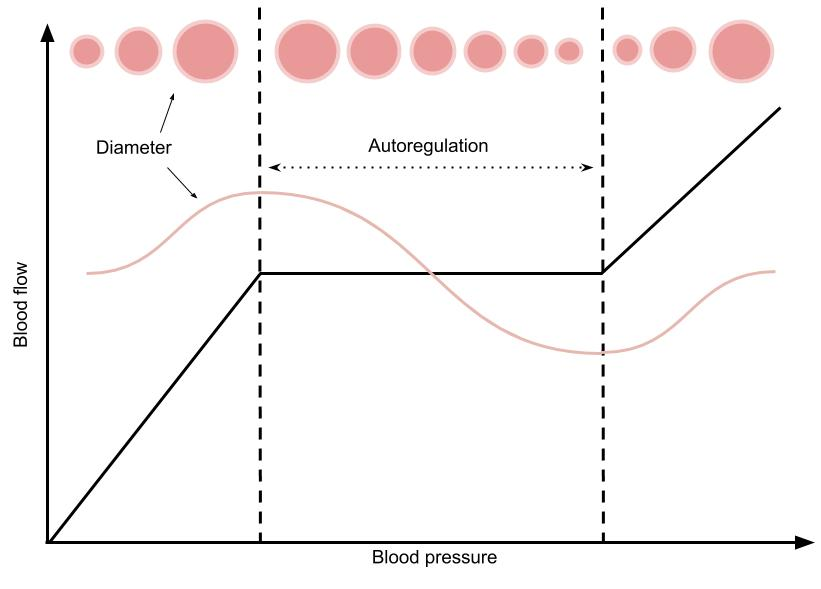
\includegraphics[width=0.6\textwidth]{fig/theory/compliance_flow.jpg}
    \caption{Pressure-flow autoregulation. The autoregulatory region is between the dashed lines, where appropriate blood flow is maintained by controlling pressure and vasodilation.}
    \label{fig:compliance_flow}
\end{figure}{}


\subsection{autoregulation} \label{sect:autoregulation}
Autoregulation is the intrinsic ability of an organ to regulate blood pressure, flow, and hence maintain appropriate perfusion. If the blood perfusion to an organ is reduced as a result of a drop in blood flow, autoregulation will return it towards normal levels within anything from 20 seconds to 3 minutes.\cite{RN19} When the body is within the autoregulatory region, between the dashed lines in figure \ref{fig:compliance_flow}, it maintains constant blood flow by regulating pressure and the resistance of the arterial system, i.e., the dilation and contraction of the blood vessels. If the blood pressure falls, the vasculature of the system will after a short period (~minute) dilate, and hence decrease the vascular resistance to regulate the relationship
\begin{equation}
    Q = P\times R
    \label{eq:pressure&flow}
\end{equation}
between pressure, flow and resistance. The reason for the slow homeostatic response of the autoregulatory system is believed to be due to slow metabolic and molecular mechanisms. The myogenic mechanism alter the ability of the vascular smooth muscle to constrict or dilate in response to differences in transmural pressure, while the release of endothelial factors, such as NO, contributes to vasodilation. \cite{RN17}

\subsubsection{Autoregulation in sepsis}\label{sect:autoregulation_sepsis}

The primary purpose of the circulatory system is to deliver oxygenated blood to tissue, where the supply of oxygen is the product of flow and oxygen content.\cite{RN11} The body has developed innate self-regulatory systems to maintain the appropriate blood flow and tissue perfusion. In a healthy individual, hemodynamic parameters fluctuate as autoregulatory mechanisms keep the cardiovascular system within a stable region. In a septic patient, however, the autoregulatory mechanisms as well as other efforts to maintain homeostasis are impaired, as the normal slow autoregulatory changes in the arterial parameters will be less stable, causing noticable changes in the impedance of the arterial system.




% Write more. https://www.cvphysiology.com/Blood%20Pressure/BP004
% Or "snapshots of hemodynamics" page 41



\section{Modeling the cardiovascular system} \label{sect:modeling}

In section \ref{sect:hemodynamics} the dynamics of blood flow, called hemodynamics, was introduced in terms of blood pressure, SVR and arterial compliance. In figure \ref{fig:windkessel_impedance} is an analogy between the fire engine Windkessel and the arterial system. The peripheral resistance of the cardiovascular system is the summed resistance of all small arteries, arterioles, and capillaries, while total arterial compliance is the sum of the compliance of all arteries. The WK model helps us understand how the arterial system functions, and is widely used for modeling the arterial system. 


\subsection{Windkessel Model} \label{sect:WK}

\begin{figure}[b!]
    \centering
    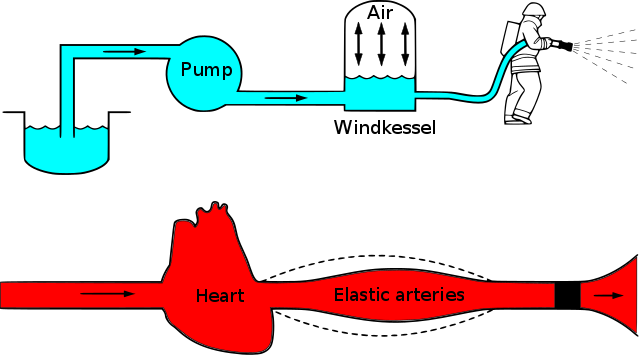
\includegraphics[width=0.7\textwidth]{fig/theory/Windkessel_effect.png}
    \caption{The analogy between a fire engine with a Windkessel from the 18th century and the artial system. The image is made by Kurzon - Own work, CC BY-SA 3.0, https://commons.wikimedia.org/w/index.php?curid=31288770}
    \label{fig:sepsis_epidemimology}
\end{figure}{}

The Windkessel model is a \textit{lumped-parameter model}, where a more accurate description of the pressure-flow relation may be acquired by including more elements. As an example, figure \ref{fig:Windkessel_circuit} shows an analogy to an electrical representation of a two- and three-element Windkessel model, where another input resistance is added to represent the characteristic impedance of the aorta \cite{RN11}, resulting in a description of the higher frequencies given by the aortic input impedance. 

Although increasing the complexity of the lumped model provides a better prediction of the relationship between pressure and flow, i.e., the impedance of the system, it becomes more challenging to determine the parameters and how much a disease like sepsis influences them. It has ,been shown that the three-element WK model inadequately estimates arterial compliance, i.e., the initial declining slope of the impedance in figure \ref{fig:windkessel_impedance}, \cite{RN18} which is one of the most important parameters when analyzing the effects of sepsis. 

\begin{figure}[t!]
    \centering
    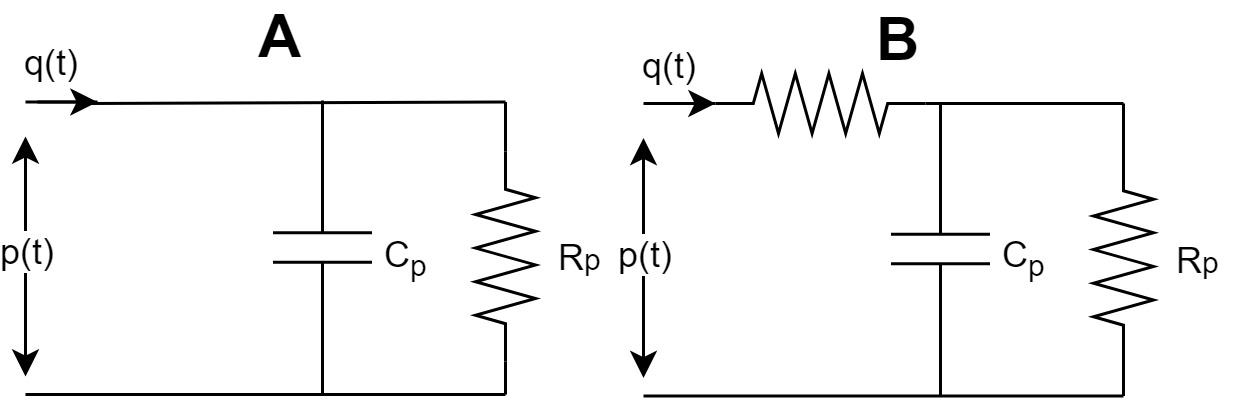
\includegraphics[width=0.8\textwidth]{fig/theory/Windkessel_circuit.jpg}
    \caption{}
    \label{fig:Windkessel_circuit}
\end{figure}{}

\subsubsection{Two-element Windkessel model}

In this project, only the two-element WK model is used. The two-element WK model assumes that the impedance of the system solely relies on peripheral resistance and total arterial compliance. By analogy to an electric circuit, all the inflow volume must be equal to the capacitance and the outflow through the resistance in figure \ref{fig:Windkessel_circuit}. The relationship between pressure and flow through the model is given by the impedance:
\begin{equation}
    Z(\omega_n) = \frac{R}{\frac{1}{R}+j\omega_n C}
    \label{eq:pressure&flow}
\end{equation}
Where R is the SVR, C the arterial compliance, and $\omega_n$ the n-th harmonic.

\begin{figure}[h!]
    \centering
    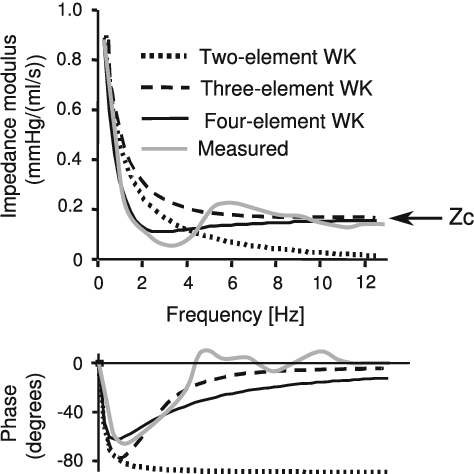
\includegraphics[width=0.6\textwidth]{fig/theory/windkessel_impedance.png}
    \caption{An example of measured aortic input impedance plotted together with impedances predicted by the two-element Windkessel, the three-element Windkessel, and the four-element Windkessel (Adapted from Westerhof et al. [76])}
    \label{fig:windkessel_impedance}
\end{figure}{}


\cleardoublepage